%! TeX program = lualatex
\documentclass[../main.tex]{subfiles}
\begin{document} \section{The limit of a function (at a number)}
  A limit describes the pattern of a function as its \emph{independent variable} moves closer to a fixed number.

  \begin{mdframed}[style=withref-compact]
    Let \(f(x)\) be a function defined at all values in an open interval containing \(a\), with the possible exception of \(a\) itself, and \(L\) be a real number. 

    If all values of the function \(f(x)\) approach the real number \(L\) as the values of \(x\) (\(\ne a\)) approach the number \(a\), then we say that \hlmain{the limit of \(f(x)\), as \(x\) approaches \(a\), is \(L\)} and denote
    \[
      L = \lim_{x \to a} f(x).
    \]

    If such number \(L\) cannot be found, then we say \hlwarn{\(\lim_{x \to a} f(x)\) does not exist}.

    \textbook{(The Intuitive) definition (of two-sided limits) on page 136}
  \end{mdframed}

  \faLightbulb{} To estimate \(\lim_{x \to a} f(x)\), we move \(x\) closer and closer to the constant \(a\) \underline{\hspace{6cm}} and look for a pattern: Does \(f(x)\) eventually get \underline{\hspace{3cm}} closer to some constant \(L\)? If such \(L\) exist, then \(L = \lim_{x \to a} f(x)\); otherwise, the limit \(\lim_{x \to a}f(x)\) does not exist.

  \begin{example}
    Consider the following functions.

    \centerline{
      \includegraphics[page=1]{../standalones/build/plot-limit-intro}
      \includegraphics[page=2]{../standalones/build/plot-limit-intro}
      \includegraphics[page=3]{../standalones/build/plot-limit-intro}
    }

    Estimate the following limits graphically:
    \begin{align*}
      \lim_{x \to 1} g_{1}(x)  
      &= \underline{\hspace{2cm}}  
      & \lim_{x \to 1} g_{2}(x) 
      &= \underline{\hspace{2cm}}
      & \lim_{x \to 1} g_{3}(x) 
      &= \underline{\hspace{2cm}} \\[2ex]
      g_{1}(1)  
      &= \underline{\hspace{2cm}}  
      & g_{2}(1) 
      &= \underline{\hspace{2cm}}
      & g_{3}(1) 
      &= \underline{\hspace{2cm}}
    \end{align*}
  \end{example}

  \faComments{} Suppose we have a function \(f(x)\), and we know \(\lim_{x \to a} f(x)\) exists. What do we know about \(f(a)\)?
  \blanklines{5}
  \clearpage

  To evaluate \(\lim_{x \to a} f(x)\) we have to approach the constant \(a\) \hlwarn{from both sides}, why not just look at it \hlsupp{one side at a time}?  Let's define \hlmain{one-sided limits}.
  \begin{itemize}
    \item If we can make \(f(x)\) arbitrarily close to a constant \(L\) by moving \(x\) closer to \(a\) \hlmain{from the left}, then we say \(\lim_{x \to a^{-}} f(x) = L\); otherwise, \(\lim_{x \to a^{-}} f(x)\) does not exist.
  
    \item If we can make \(f(x)\) arbitrarily close to a constant \(L\) by moving \(x\) closer to \(a\) \hlmain{from the right}, then we say \(\lim_{x \to a^{+}} f(x) = L\); otherwise, \(\lim_{x \to a^{+}} f(x)\) does not exist.
  \end{itemize}
  
  \begin{example}
    Let's look at \(g_{1}(x)\) and \(g_{2}(x)\) again.

    \begin{center}
      \begin{tikzpicture}[scale=1]
        \begin{axis}[title={\(g_{1}(x)\)}, 
          ]
          \addplot[thick] {-(x-1)^3 + 1};
          \draw[fill=white] (axis cs:1,1) circle (0.05);
          \draw[fill=black] (axis cs:1,2) circle (0.05);
        \end{axis}
      \end{tikzpicture}
      \hspace{1in}
      \begin{tikzpicture}[scale=1]
        \begin{axis}[title={\(g_{2}(x)\)}, 
          ]
          \addplot[thick, domain=-2:1] {x};
          \addplot[thick, domain=1:2] {2};

          \draw[fill=white, thick] (axis cs:1,1) circle (0.05);
        \end{axis}
      \end{tikzpicture}
    \end{center}

    Estimate the following one-sided limits.
    \begin{align*}
      \lim_{x \to 1^{-}} g_{1}(x) 
      &= \underline{\hspace{2cm}}
      & \lim_{x \to 1^{-}} g_{2}(x) 
      &= \underline{\hspace{2cm}} \\[2ex]
      \lim_{x \to 1^{+}} g_{1}(x) 
      &= \underline{\hspace{2cm}}
      & \lim_{x \to 1^{+}} g_{2}(x) 
      &= \underline{\hspace{2cm}}
    \end{align*}
  \end{example}
  
  \begin{mdframed}[style=withref-compact]
    Supppse \(f(x)\) is defined at all values in an open interval containing some constant \(a\) with the possible exception of \(a\) itself, and let \(L\) be a real number. Then
    \[
      \lim_{x \to a} f(x) = L \qquad\text{if and only if}\qquad \lim_{x \to a^{-}} f(x) = L \text{ and } \lim_{x \to a^{+}} f(x) = L.
    \]
    \textbook{Theorem 2.2 on page 145}
  \end{mdframed}
  
  \begin{itemize}[topsep={1ex}]
    \item If we know \underline{\hspace{2in}}, then conclude \underline{\hspace{3in}}.
      \vfill{}

    \item If we know \underline{\hspace{2in}}, then conclude \underline{\hspace{3in}}.
      \vfill{}
    \item If we know \underline{\hspace{2in}} or one of them does not exist, then conclude that 
      \vfill{}
  \end{itemize}
  \clearpage
  

  Textbook Theorem~2.2 shows one way that a limit fails to exists: When its left and right limits don't agree. How else can a limit fail to exist?

  \begin{example} \label{ex:limit-sin-1/x}
    Does \(\lim_{x \to 0} \sin \left(\frac{1}{x}\right) \) exist? Support your reasoning using a graph or a table of values.

    \blanklines{5}
  \end{example}

  \begin{example}
    Come up with a function \(f(x)\) whose \( \lim_{x \to 0^{+}} f(x)\) does not exist. Explain why your answer is correct. 

    \blanklines{5}
  \end{example}

  A limit can fail to exist if a function ``goes to infinity'' at \(a\). This is called an \hlmain{infinite limit}. 

  There are four possibilities.
  \begin{center}
    \begin{tikzpicture}
      \begin{axis}[title={\(h_{1}(x)\)}]
        \addplot[thick, smooth, domain=-2:0.99] {(1/4)/(x-1) + 1};
        \addplot[thick, smooth, domain=1.01:3] {(1/4)/(x-1) - 1};
        \addplot[dotted] coordinates { (1,3) (1,-3) };
      \end{axis}
    \end{tikzpicture}
    \begin{tikzpicture}
      \begin{axis}[title={\(h_{2}(x)\)}]
        \addplot[thick, smooth, domain=-2:0.99] {-(1/4)/(x-1)};
        \addplot[thick, smooth, domain=1.01:3] {-(1/4)/(x-1)};
        \addplot[dotted] coordinates { (1,3) (1,-3) };
      \end{axis}
    \end{tikzpicture}
    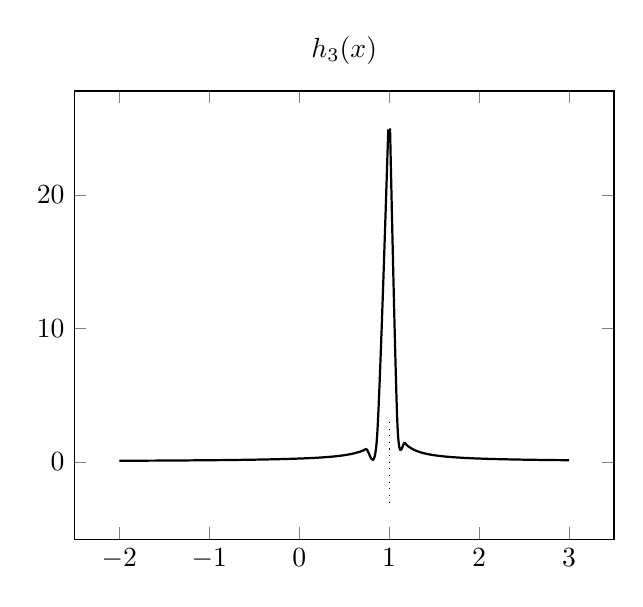
\begin{tikzpicture}
      \begin{axis}[title={\(h_{3}(x)\)}]
        \addplot[thick, smooth, domain=-2:0.99] {-(1/4)/(x-1)};
        \addplot[thick, smooth, domain=1.01:3] {(1/4)/(x-1)};
        \addplot[dotted] coordinates { (1,3) (1,-3) };
      \end{axis}
    \end{tikzpicture}
    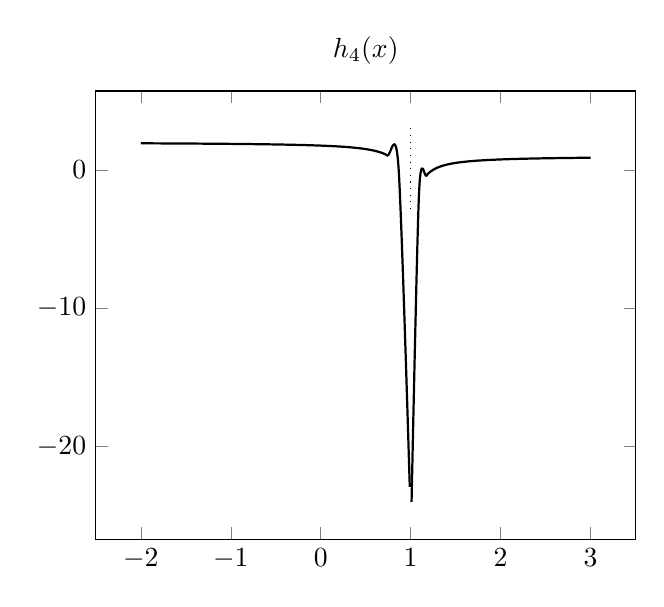
\begin{tikzpicture}
      \begin{axis}[title={\(h_{4}(x)\)}]
        \addplot[thick, smooth, domain=-2:0.99] {(1/4)/(x-1) + 2};
        \addplot[thick, smooth, domain=1.01:3] {-(1/4)/(x-1) + 1};
        \addplot[dotted] coordinates { (1,3) (1,-3) };
      \end{axis}
    \end{tikzpicture}
  \end{center}
  \begin{align*}
    \lim_{x \to 1^{-}} h_{1}(x) 
    &= \underline{\hspace{1cm}} 
    & \lim_{x \to 1^{-}} h_{2}(x) 
    &= \underline{\hspace{1cm}} 
    & \lim_{x \to 1^{-}} h_{3}(x) 
    &= \underline{\hspace{1cm}} 
    & \lim_{x \to 1^{-}} h_{4}(x) 
    &= \underline{\hspace{1cm}} \\[2ex]
    \lim_{x \to 1^{+}} h_{1}(x) 
    &= \underline{\hspace{1cm}} 
    & \lim_{x \to 1^{+}} h_{2}(x) 
    &= \underline{\hspace{1cm}} 
    & \lim_{x \to 1^{+}} h_{3}(x) 
    &= \underline{\hspace{1cm}} 
    & \lim_{x \to 1^{+}} h_{4}(x) 
    &= \underline{\hspace{1cm}} \\[2ex]
    \lim_{x \to 1} h_{1}(x) 
    &= \underline{\hspace{1cm}} 
    & \lim_{x \to 1} h_{2}(x) 
    &= \underline{\hspace{1cm}} 
    & \lim_{x \to 1} h_{3}(x) 
    &= \underline{\hspace{1cm}} 
    & \lim_{x \to 1} h_{4}(x) 
    &= \underline{\hspace{1cm}}
  \end{align*}
  
  A vertical line \(x = a\) is called a \hlmain{vertical asymptote} of \(f(x)\) if
  \[
    \lim_{x \to a^{-}} f(x) = \pm \infty \qquad\text{ or }\qquad \lim_{x \to a^{+}} f(x) = \pm \infty.
  \]
  \blanklines{7}
  \clearpage

  Theorem~2.3 boils down to just two pictures.
  \begin{center}
    \begin{tikzpicture}
      \begin{axis}[title={\(\textstyle \frac{1}{(x-a)^{n}}\) if \(n\) is odd},
        xtick={1}, xticklabel={\(a\)}
        ]
        \addplot[thick, smooth, domain=-2:0.99] {(1/4)/(x-1)};
        \addplot[thick, smooth, domain=1.01:3] {(1/4)/(x-1)};
        \addplot[dotted] coordinates { (1,3) (1,-3) };
      \end{axis}
    \end{tikzpicture}
    \hspace{1in}
    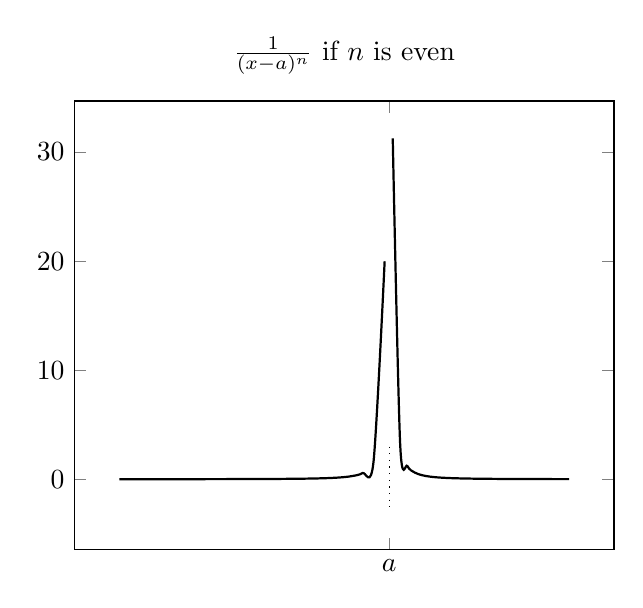
\begin{tikzpicture}
      \begin{axis}[title={\(\textstyle \frac{1}{(x-a)^{n}}\) if \(n\) is even},
        xtick={1}, xticklabel={\(a\)}
        ]
        \addplot[thick, smooth, domain=-2:0.95] {(1/20)/(x-1)^2};
        \addplot[thick, smooth, domain=1.04:3] {(1/20)/(x-1)^2};
        \addplot[dotted] coordinates { (1,3) (1,-3) };
      \end{axis}
    \end{tikzpicture}
  \end{center}

  \blanklines{25}

  % We will skip Theorem~2.3 in the textbook for now. There is no need to memorize such table. We will learn a very simple technique to identify vertical asymptotes algebraically after we learn limit laws. 
  %
  % Here is the technique for the impatient. We know \(\frac{1}{(x-a)^{n}}\) has a vertical asymptote from our review of sketching graphs. The only thing left is to decide the sign of the infinity in these limits:
  % \[
  %   \lim_{x \to a^{-}} \frac{1}{(x-a)^{n}} = (\hlsupp{\text{pos or neg?}})\,\infty 
  %   \hspace{1in}
  %   \lim_{x \to a^{+}} \frac{1}{(x-a)^{n}} = (\hlsupp{\text{pos or neg?}})\,\infty.
  % \]
  %
  % \begin{itemize}
  %   \item For \(\lim_{x \to a^{-}}\), evaluate the function at a number \(b\) very close to \(a\) but to the left of \(a\) (meaning smaller than \(a\)), say \(b = a - 0.001\). The one-sided limit has the same sign as \(f(b)\).
  %   \item For \(\lim_{x \to a^{+}}\), evaluate the function at a number \(b\) very close to \(a\) but to the right of \(a\) (meaning larger than \(a\)), say \(b = a + 0.001\). The one-sided limit has the same sign as \(f(b)\).
  % \end{itemize}


  % Vertical asymptotes have a very subtle trap!
  % \begin{example}
  %   Let \(f(x) = \frac{6x^{2} + 19 x + 10}{2x + 5}\).  Is \(x = -5/2\) a vertical asymptote of \(f(x)\)?
  % \end{example}
  
  Here is a variation-on-the-theme exercise.
  \begin{example}
    A function \(f(t)\) is represented by a table of values below. Estimate \(\lim_{t \to 0} f(x)\).

    \hspace{2in} \includegraphics{../standalones/build/table_t_squared}
  \end{example}

\end{document}
